% !TeX spellcheck = de_DE
\documentclass{alex_gp}
\usepackage[export]{adjustbox}

\name{Alexander Helbok}
\course{Grundpraktikum}
\hwnumber{6}
\spacing{}


\begin{document}
\renewcommand{\labelenumi}{\alph{enumi})}


\begin{mybox}{Stärke und Inklination des Erdmagnetfeldes}
	Ziel dieses Versuches ist es, sowohl den Betrag, als auch die Ausrichtung des Erdmagnetfeldes in Innsbruck zu bestimmen. Dafür wird der Magnetsensor des IOLab verwendet, welcher zuerst kalibriert werden muss. 
	
	Der Magnetsensor misst das Magnetfeld ich die drei (kartesischen) Raumrichtungen. Um die Berechnung der Magnitude und Inklination des Magnetfeldes zu vereinfachen, drehen wir unser Koordinatensystem (das IOLab) so, dass der Sensor im Rahmen der Unsicherheit einen Wert von 0 in eine Raumrichtung ausgibt. In unserem Fall war das die y-Komponente, welche minimiert wurde. Dann ergibt sich nämlich für den Gesamtbetrag des Erdmagnetfeldes 
	\begin{equation}\label{eqn:mag1}
		|\vec{B}| = \sqrt{B_x^2 + B_z^2}
	\end{equation}
	und für den Inklinationswinkel
	\begin{equation}\label{eqn:theta1}
		\theta = \arctan(\tfrac{B_z}{B_x})
	\end{equation}
	
	Die Messung wurde am Boden durchgeführt und lief etwas über \( 30 \unit{s} \). Die gewonnen Daten sind in \autoref{fig:Bmean} dargestellt. Es wurde für jede Komponente der Mittelwert gebildet und der Fehler auf die Standardabweichung gesetzt, da dann (per Definition) zwei drittel der Daten innerhalb des \( 1\sigma \) Intervalls liegen. 
	
	\begin{figure}[H]	
		\centering
		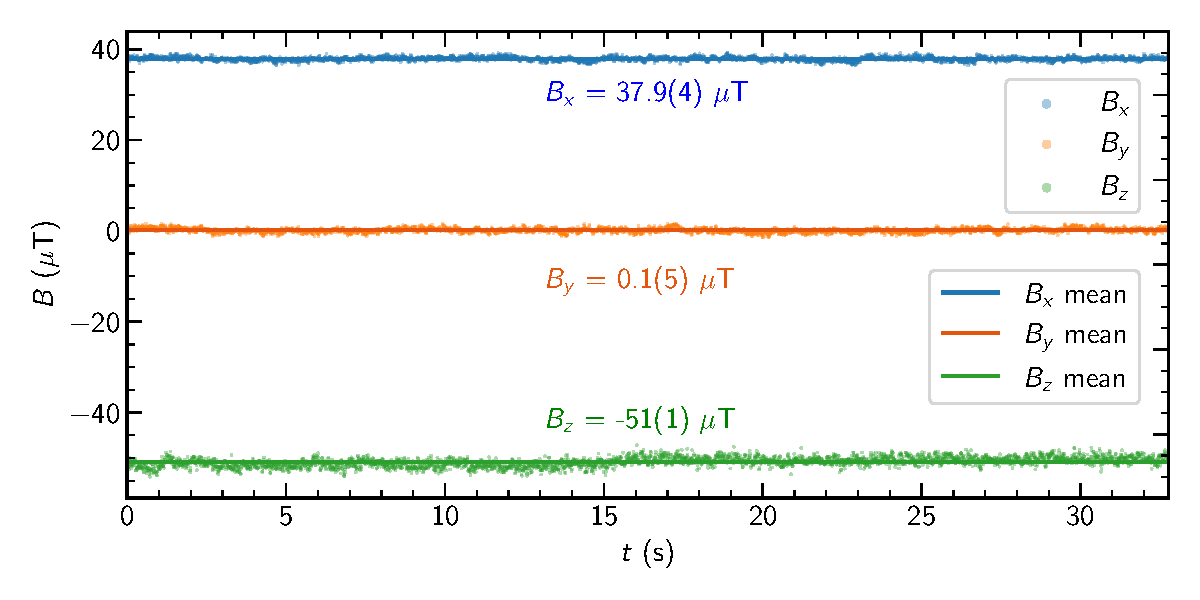
\includegraphics[width=\textwidth]{Versuch6_1}
		\caption{Das gemessene Magnetfeld in die drei kartesischen Raumrichtungen farblich unterscheidbar auf die Zeit aufgetragen. Der Mittelwert der Daten wird als durchgezogene Linie dargestellt.}
		\label{fig:Bmean}
	\end{figure}
	
	Man erhält für die drei kartesischen Komponenten des Erdmagnetfeldes
	\begin{equation}\label{eqn:Bxyz}
		B_x = 37.9(4) \unit{\micro T} \qquad B_y = 0.1(5) \unit{\micro T} \qquad B_z = -50.9(1.0) \unit{\micro T}
	\end{equation}

	Daraus lässt sich jetzt mit \autoref{eqn:mag1} und \autoref{eqn:theta1} die Stärke und Inklination des Erdmagnetfeldes berechnen und man erhält folgende Werte
	\begin{equation}\label{eqn:results}
		|\vec{B}| = 63.4(9) \unit{\micro T} \hspace{3cm} \theta = \ang{53.3(6)}
	\end{equation}
	
	Vergleicht man diese Werte mit Literaturwerten \footnotemark[1]
	\begin{equation}\label{key}
		|\vec{B}| = 48.40(15) \unit{\micro T} \hspace{3cm} \theta = \ang{63.5(2)}
	\end{equation}
	erkennt man, dass unsere gemessenen Werte signifikant abweichen. Das liegt wahrscheinlich daran, dass am Versuchsort eine Vielzahl an metallische Objekte vorhanden waren, die Magnetfelder beeinflussen oder sogar selber erzeugen. Der Versuch wurde nämlich in einem Gebäude aus Stahlbeton durchgeführt, in einem Raum voller Elektronik und oberhalb Labore, in welchen Experimente mit elektrischen und Magnetische Felder durchgeführt werden. Es kommt daher zu systematischen Abweichungen, die verringert werden können, indem man die Messung fern von metallischen Objekten wiederholt.

	\footnotetext[1]{https://www.ngdc.noaa.gov/geomag/calculators/magcalc.shtml\#igrfwmm}
\end{mybox}

\begin{mybox}{Elektromotor}
	In diesem Versuch wird mithilfe der Lorentz Kraft die Polung eines Permanentmagneten bestimmen. Der Versuchsaufbau sah wie folgt aus: Auf den Magneten wurde eine leitende Schraube gestellt, dessen Spitze als Drehachse fungiert. Auf die Schraubenspitze balancieren wir eine Batterie. Das andere Ende der Batterie verbinden wir mit einem Kabel mit dem Magneten. Hierbei ist wichtig, das Kabel am äußeren Rand des Magneten anzuschließen, da es sonst zu keiner Rotation der Batterie kommt.
	
	Die Lorentz Kraft ist so definiert 
	\begin{equation}\label{eqn:Fl}
		\vec{F} = q \vec{v} \times \vec{B}
	\end{equation}
	mit der Ladung \( q \), der Geschwindigkeit der Ladungen \( \vec{v} \) und dem Magnetfeld \( \vec{B} \). Das Magnetfeld in einem Permanentmagneten verläuft annähernd geradlinig vom Südpol zum Nordpol. Das Kreuzprodukt wird maximal, wenn die beiden Vektoren normal aufeinander stehen, also wenn der Strom seitlich in (oder aus) den Magneten fließt, weshalb das Kabel auch an der Seite angebracht wurde. 
	
	Je nach Ausrichtung des Magneten geht das Magnetfeld in die positive oder negative z-Richtung und je nach Ausrichtung der Batterie fließt der Strom von der Batterie über das Kabel in den Magneten oder umgekehrt (das Koordinatensystem wurde so gelegt, dass der Strom in der xz-Ebene fließt). Wir haben also vier verschiedene Konfigurationsmöglichkeiten mit zwei unterschiedliche Beobachtungen, eine Drehung in und gegen den Uhrzeigersinn. In \autoref{fig:Motor} ist der Versuchsaufbau (links), sowie die möglichen Konfigurationsarten (rechts) dargestellt.
	
	\begin{figure}[H]
		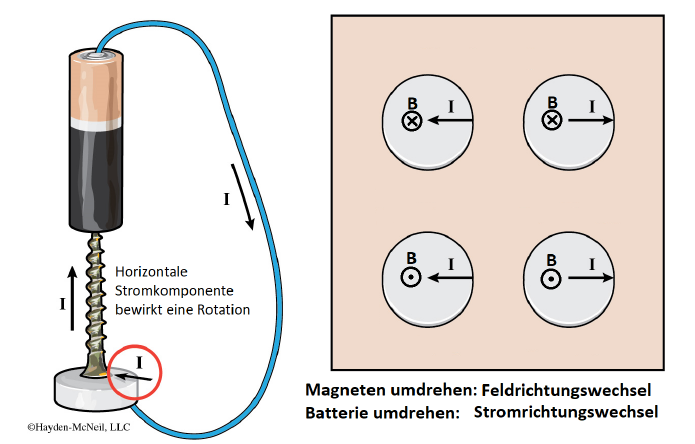
\includegraphics[width=.7\textwidth, right]{Motor}
		\caption[]{Links: Versuchsaufbau des Batteriemotors. Auf einen Permanentmagneten wird über eine Schraube eine Batterie gestellt, welche über ein Kabel wieder mit dem Magneten in der Basis verbunden ist. Rechts: möglichen Konfigurationsarten des Versuchs mit eingezeichnetem Strom und Magnetfeld. Graphik entnommen aus \footnotemark[2] }
		\label{fig:Motor}
	\end{figure}
	
	\begin{minipage}{\textwidth}
		\vspace{-13cm}
		\begin{tikzpicture}[scale=3]
			\draw[-Stealth] (0,0) -- (0,1) node [above] {\large \( z \)};
			\draw[-Stealth] (0,0) -- (1,0) node [right] {\large \( x \)};
			\draw[-Stealth] (0,0) -- (0.6,0.4) node [right] {\large \( y \)};
			
			\node at (3.2,1.8) {\large \( 1 \)};
			\node at (4,1.8) {\large \( 2 \)};
			\node at (3.2,0.9) {\large \( 3 \)};
			\node at (4,0.9) {\large \( 4 \)};
		\end{tikzpicture}
	\end{minipage}

	Anhand der Stromrichtung und der Drehung kann man auf die Richtung des Magnetfeldes schließen, da auf die bewegten Ladungsträger (der Strom) dir Lorentz Kraft wirkt und die Batterie zum Drehen bringt. Das Vorzeichen der Ladungsträger spielt keine Rolle, da sich dann neben dem Vorzeichen von \( q \) auch die Flussrichtung ändern würde, was sich wegkürzt. Man kann mit diesem Experiment also nicht herausfinden, welches Vorzeichen die Ladungsträger des elektrischen Stromes haben. Der Versuch wurde viermal durchgeführt und die Ergebnisse sind in \autoref{table:1} eingetragen. Die Strom- und Drehrichtung wurden beobachtet, woraus sich die Magnetfeldrichtung erschließt. Die Konfigurationen wurden dann mit \autoref{fig:Motor} verglichen und gematched. 
	
	\begin{center}
		\captionof{table}{Stromrichtung, Drehrichtung und daraus erschlossene Magnetfeldrichtung für die vier Konfigurationen.}
		\begin{tabular}{@{\extracolsep{5mm}} 
				r
				c
				c
				c
			}
			\toprule
			\makecell[t]{Konfiguration}
			&   {\makecell[t]{Stromrichtung}}
			&   {\makecell[t]{Drehrichtung}}
			&   {\makecell[t]{Magnetfeldrichtung}}\\
			\midrule
			1 & \( -\hat{x} \) & \( \circlearrowright \) & \( -\hat{z} \) \\
			2 & \( \phantom{-}\hat{x} \) & \( \circlearrowleft \) & \( -\hat{z} \) \\
			3 & \( -\hat{x} \) & \( \circlearrowleft \) & \( \phantom{-}\hat{z} \) \\
			4 & \( \phantom{-}\hat{x} \) & \( \circlearrowright \) & \( \phantom{-}\hat{z} \) \\
			\bottomrule
		\end{tabular}
		\label{table:1}
	\end{center}
	\footnotetext[2]{Angabe}
\end{mybox}

\begin{mybox}{Strom durch Leiter}
	Ziel dieses Versuches ist es, den Strom in einem Leiter anhand vom erzeugten Magnetfeld zu bestimmen. Dafür wurde eine frische Batterie über ein Kabel der Länge \( d = 2.97(1) \unit{m} \) kurzschlossen und das erzeugte Magnetfeld mit dem Magnetfeldsensor vom IOLab aufgezeichnet. Diese Messung wurde 11 Mal durchgeführt, wobei nach jedem Durchgang das IOLab um \( 1.0 (1) \unit{cm} \) vom Leiter wegbewegt wurde. 
	
	Der Magnetsensor im IOLab ist in einer Höhe von \( H = 2.0(1) \unit{cm} \) und einer Tiefe von \( T = 0.9(1) \unit{cm} \) verbaut. Der effektive Abstand vom Leiter ergibt sich dann aus 
	\begin{equation}\label{eqn:r}
		r = \sqrt{H^2+T^2+R^2}
	\end{equation}
	wobei \( R \) nach jedem Durchgang um \( 1.0(1) \unit{cm} \) erhöht wird.
	
	In \autoref{fig:Bcable} sind die aufgezeichneten Daten für die drei Raumkomponenten zu sehen. In x-Richtung sind keine Ausschläge zu sehen, da diese Achse parallel zum Leiter war und das Magnetfeld radial um den Leiter geht und keine parallele Komponente besitzt. In den anderen 2 Raumrichtungen sieht man 11 Ausschläge, die mit der Zeit an Magnitude abnehmen, da das IOLab ja immer weiter wegbewegt wurde und das gemessene Magnetfeld vom Leiter daher auch weniger stark war.
	
	\begin{figure}[H]	
		\centering
		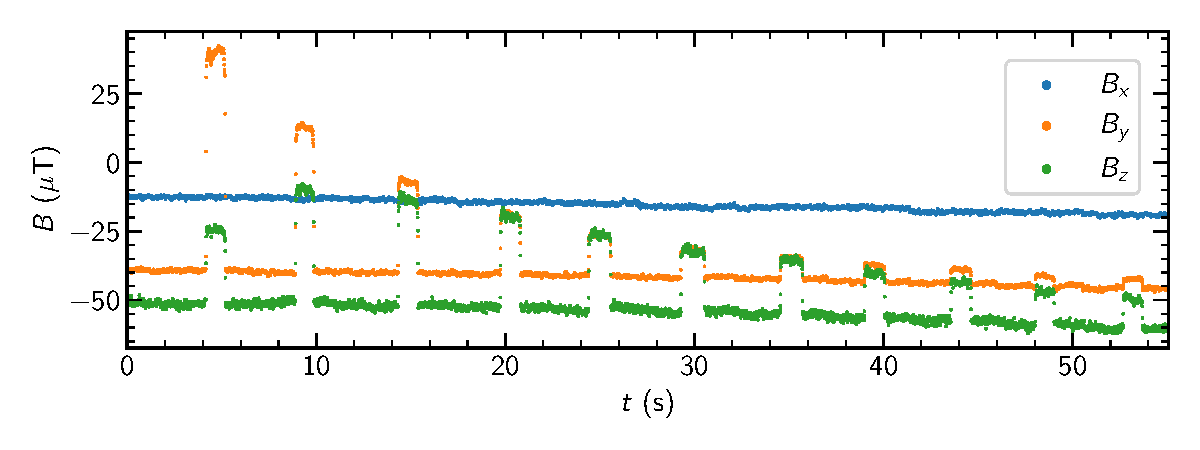
\includegraphics[width=\textwidth]{Versuch6_3}
		\caption{Das gemessene Magnetfeld in die drei kartesischen Raumrichtungen farblich unterscheidbar auf die Zeit aufgetragen. Der Mittelwert der Daten wird als durchgezogene Linie dargestellt.}
		\label{fig:Bcable}
	\end{figure}
	
	Die Analyse der Daten ging wie folgt: Die Ausschläge wurden ermittelt und in diese wurde eine Konstante gelegt.	Von den Maxima muss noch der Untergrund abgezogen werden, um die vom Strom verursacht Änderung vom Magnetfeld zu bestimmen. Dafür wurde 2 Sekunden vor und nach dem Ausschlag die Daten gemittelt und aus diesen beiden Werten wieder der Mittelwert gebildet. Jetzt kann man die relative Änderung und daraus über die Wurzel der Quadratsummen (Siehe \autoref{eqn:mag1}) die Stärke des Magnetfeldes bestimmen. 
	
	Der Absolutbetrag des Magnetfeldes ist gegeben durch 
	\begin{equation}\label{eqn:last}
		|\vec{B}(r)| = \frac{\mu_0 I}{2\pi}\frac{1}{r} = k\tilde{r}
	\end{equation}
	wobei der konstante Vorfaktor durch \( k := \tfrac{\mu_0 I}{2\pi} \) ersetzt wurde. Da man aus Geraden leichter Werte, wie die Steigung ablesen kann, wurde \( \tilde{r} := 1/r \) eingeführt. Wir erwarten uns also, dass die Magnetfeldstärke proportional zum Kehrwert des Abstandes ist und aus der Konstante lässt sich dann der Strom ermitteln. In \autoref{fig:BFit} die Änderung der Magnetfeldes \( \Delta B \) auf den Kehrwert des Abstands \( \tilde{r} \) aufgetragen und es ist eine Gerade in rot angepasst. Die Gerade geht gezielt durch den Ursprung, da wir bei einem Abstand von \( \infty \) (und daher einem Kehrwert von 0) kein Magnetfeld zu spüren. Des weiteren erhöht das die Anzahl der Freiheitsgrade von 9 auf 10, was bei dem Fit nicht von großer Bedeutung ist, da die Daten nicht wirklich zum Fit passen. 
	
	\begin{figure}[H]	
		\centering
		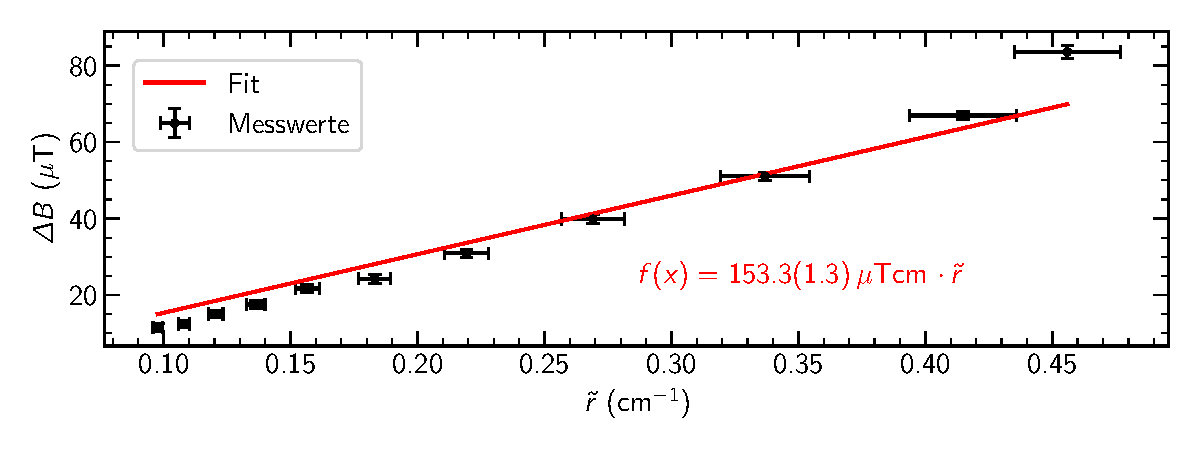
\includegraphics[width=\textwidth]{Versuch6_4}
		\caption{Die gemessene Magnetfeldänderung für verschiedene Abstände. Eine Gerade wurde in rot an die Daten angepasst.}
		\label{fig:BFit}
	\end{figure}

	Für die Steigung der Gerade erhält man einen Wert von \( k = 153.3(1.3) \unit{\micro\tesla\cm} \), woraus sich mit \autoref{eqn:last} ein Strom von \( I = 7.67(7) \unit{A} \) ergibt.
	
	Nimmt man für die Batterie eine Spannung von \( U = 1.5(1) \unit{V} \) und einen Innenwiderstand von \( R_{\text{Batt}} = 0.15 \unit{\ohm} \) und für das Kabel einen Leitwiderstand von \( R_{\text{lw}} = 40.1 \unit{\ohm/km} \) an, kann man sich mithilfe des Ohmschen Gesetzes \( I = U/R \) den fließenden Strom berechnen. Setzt man hier Werte ein erhält man \( I_{\text{calc}} = 5.6(4) \unit{A} \).
	
	Unser Wert weicht also deutlich vom theoretischen Wert ab, was an mehreren Sachen liegen kann. Einerseits entlädt sich die Batterie bei einem Kurzschluss rapide, wodurch sich die Spannung und damit der fließende Strom reduziert. Um den Strom zeitlich konstant zu halten, müsse man eine andere Spannungsquelle verwenden, die direkt am Stromnetz hängt und sich daher nicht entlädt. Zweitens wurde der Versuch in einem Gebäude voller metallischer Gegenstände durchgeführt, welche das vom Leiter erzeugt Magnetfeld verzerren. Um dieses Problem zu beheben, müsste man den Versuch an einem Ort durchführen, der möglichst Metallfrei ist. 
	
	In der Berechnung vom Strom ist die größte Fehlerquelle die Messung des Magnetfeldes, da die Ausschläge nur sehr kurz sind und die Werte im Peak streuen. Das Problem könnte man mit einer kontinuierlichen und vor allem konstanten Stromquelle beheben, dann müsste man den Stromfluss gar nicht mehr unterbrechen, sonder könnte bei fließendem Strom den Abstand des IOLabs erhöhen.
\end{mybox}


\end{document}